\documentclass[../main]{subfiles} \begin{document}

\chapter{引言}%
\label{cha:引言}

二十一世纪是光子的时代,是信息的社会,随着信息技术的飞速发展,人们获取信息的手段
在向不同波段,更广阔的领域扩展;红外成像技术正是顺应了这一时代的发展趋势,已经成
为当今世界发达国家大力发展的军民两用的新兴高科技之一。由于西方发达国家对我国高技
术的封锁,加上我国红外成像研究起步较晚,基础理论研究和材料工艺比较落后,所以目前
国产的红外焦平面阵列探测器和红外成像系统整机的性能与发达国家相比还有一定差距。因
此,红外成像的基础理论及其关键技术的研究对提升红外成像技术在我国国防建设和国民经
济各领域的应用比重,缩小我国在该领域与发达国家的差距有着非常重要的意义。

红外探测器的非均匀性是限制其性能与应用的首要因素。这种非均匀性表现为一种叠加在图
像上固定图案噪声。造成这种非均匀性的原因很多。

红外焦平面阵列非均匀性的主要因素是每个探测器单元的响应率的不一致性。红外焦平面阵
列由数万个像元构成,由于各个像元的响应参数不尽相同,造成即使在均匀输入的情况下,
各个像素的响应也不一致。如图\ref{fig:像元响应曲线}所示。

\begin{figure}[htbp]
\centering
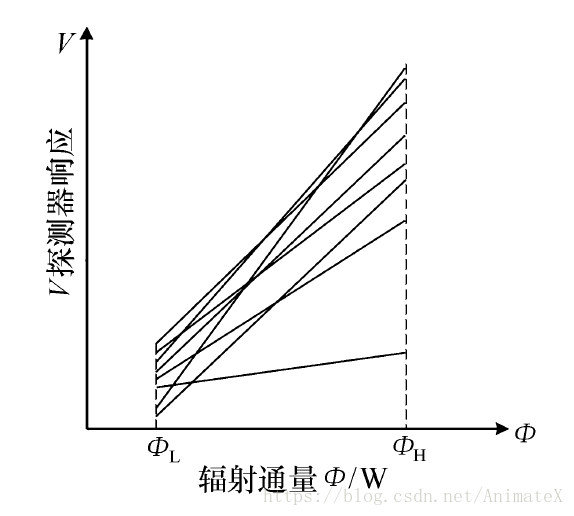
\includegraphics[width=0.4\linewidth]{reponse.png}
\caption{像元响应曲线}
\label{fig:像元响应曲线}
\end{figure}

其次是探测器读出电路自身以及读出电路和探测器的耦合因素等。此外研究发现,红外探测
器非均匀性的时间稳定性不佳,会随着工作时间的增加与外界环境的改变而缓慢漂移,严重
影响图像的空间分辨率与温度灵敏度。所以,红外探测器必须采用相应的非均匀性校正措施
,来修正这种探测器不均匀响应造成的影响。

常见的校正算法主要分为两大类:

\begin{enumerate}
	\item 基于定标的非均匀性校正
	\item 基于场景的非均匀性校正
\end{enumerate}

\end{document}

